В результате пьезоэлектрического эффекта происходит деформация
кристаллической решетки. Данный эффект, очевидно, будет влиять на
КДО, а именно, на ее угловое положение и профиль.
Изменение профиля КДО может быть вызвано несколькими физическими процессами:

1. Изменение профиля может происходить за счет изменения структурного фактора при
пьезоэффекте. Данный эффект не рассматривается в рамках настоящей работы.
В первом приближении можно ограничиться случаем однородной деформации решетки
 кристалла. Такая деформация описывается
 матрицей пьезомодулей, вследствие чего относительное расположение атомов
 внутри элементарной ячейки остается постоянным, как и структурный фактор.

 \begin{figure}[H]
   \centering
   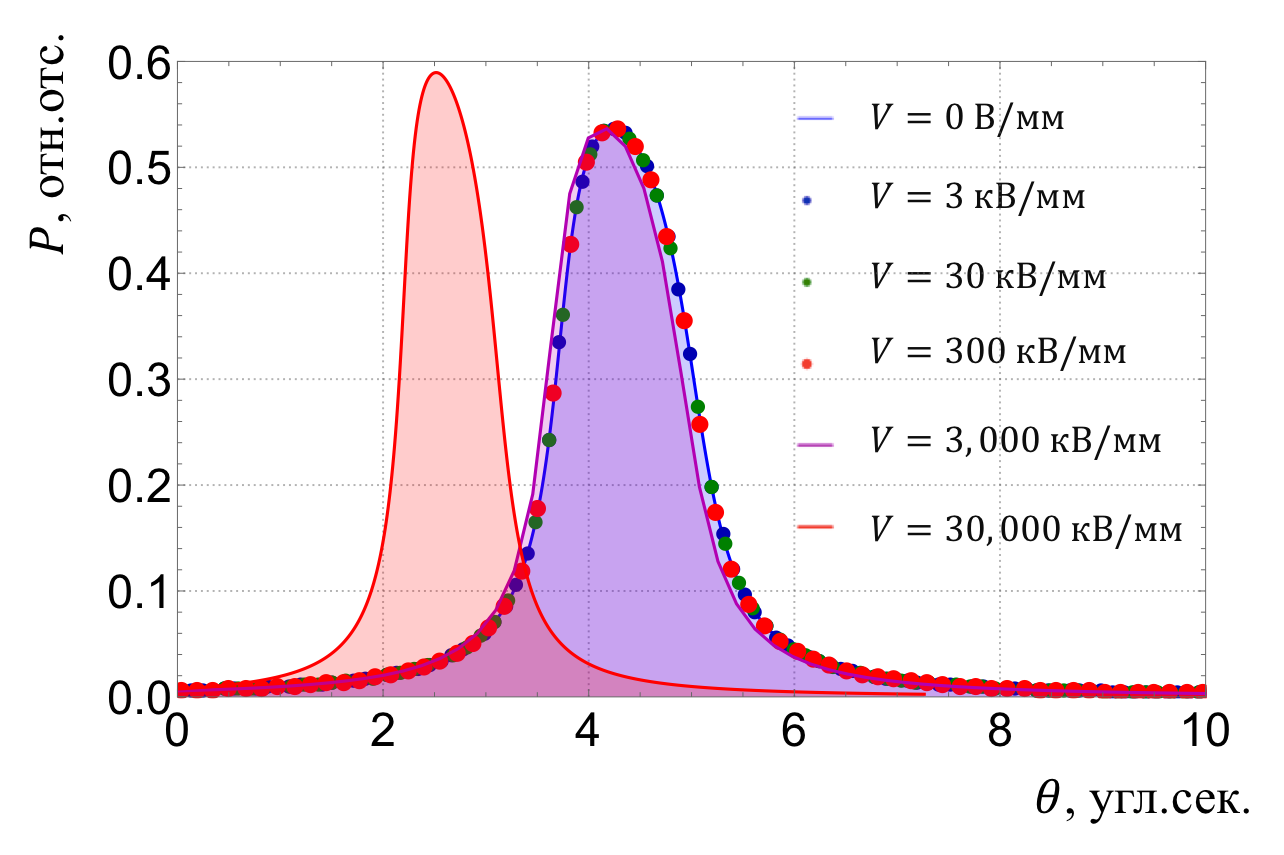
\includegraphics[width=0.6\textwidth]{images/self_kdo_under_ex_field.png}
   \caption{Изменение профиля собственной КДО для кристалла LGT(220)
   в зависимости от величины внешнего электрического поля}
   \label{ris:self_kdo_deformation}
 \end{figure}

Стоит отметить, что учет анизатропии деформации решетки, вызванный различной чувствительностью
атомов разных сортов к электрическому полю, является актуальной и интересной задачей,
решение которой с помощью рентгеновской дифракции может стать существенным шагом
на пути понимания природы пьезоэффекта.

2. Профиль кривой также может изменяться вследствие изменения степени
 дисперсионности экспериментальной схемы.
При пьезоэффекте меняется межплоскостное расстояние образца, а значит и его угол Брэгга.
Таким образом, может возникать дисперсионное уширение или сужение КДО и изменение интегральной интесивности
отраженного пучка (см. \ref{sec:dispersion_cal_an_exp}) в зависимости
от увеличения или уменьшения разности углов Брэгга образца и монохроматора
по воздействием внешнего электрического поля. Для оценки этого эффект был
проведен расчет, который заключался в оценке полуширины результирующей двухкристальной КДО
в зависимости от параметра решетки образца и, как следствие
 изменения угла Брэгга (рис. \ref{ris:FWHM_diference_bragg}).
%(отлажить по оси х дельта брэгга)
\begin{figure}[H]
  \centering
  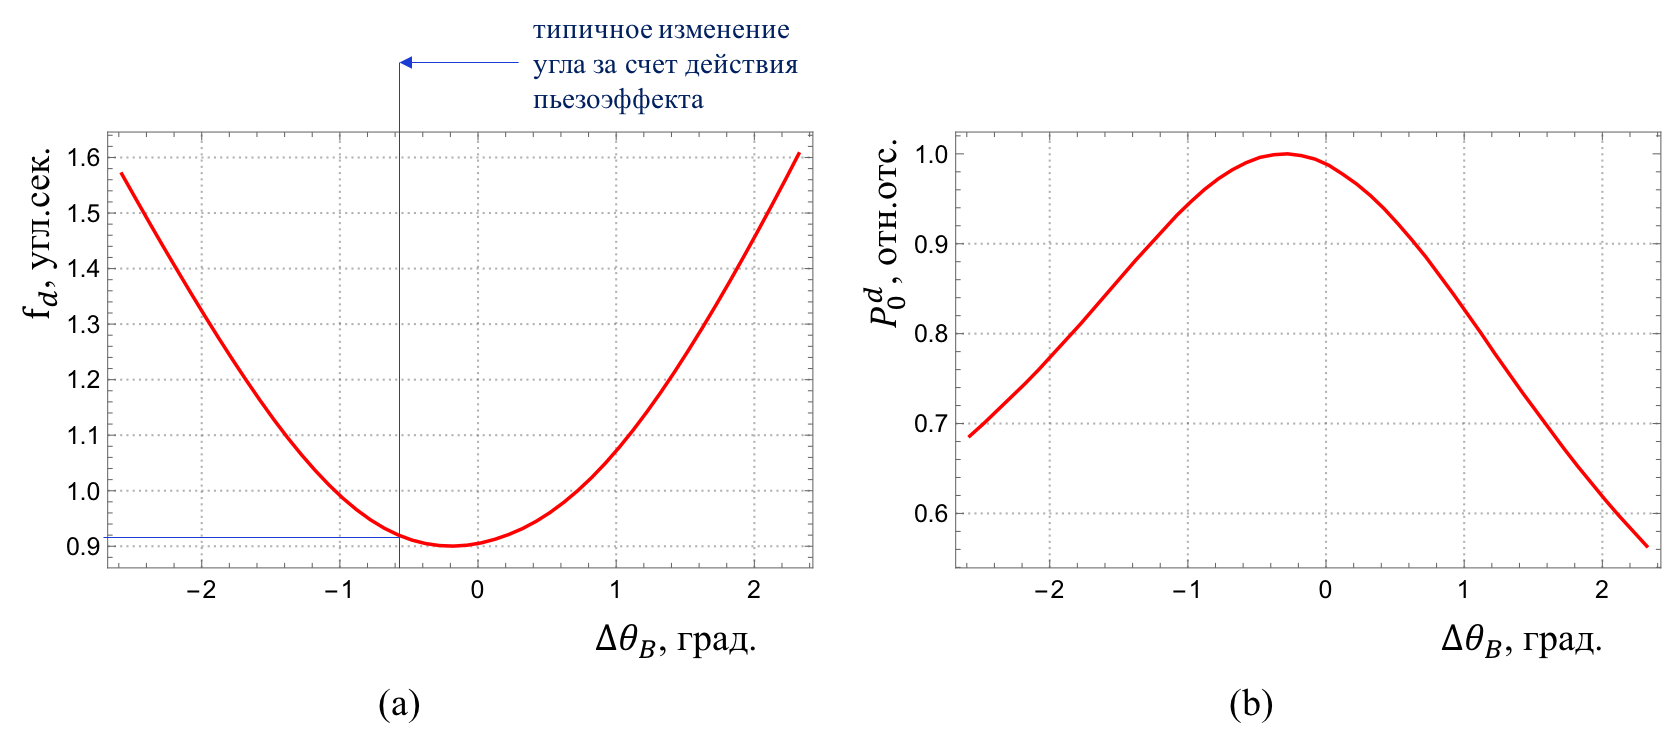
\includegraphics[width=0.95\textwidth]{images/delta_bragg_dispers.png}
  \caption{Зависимость (a) полуширины двухкристальной КДО $f_d$ и (b) амплитуды в максимуме КДО  $P^d_0$
   от разности углов Брэгга $\Delta\theta_B =\theta_B^S-\theta_B^M $ кристаллов
  образца (S) и монохроматора (M). Отсчет ведется от угла Брэгга моноохроматора $\theta_B^M = 21.6785 ^o$ - Si (440),
  в качестве образца был взят кристалл LGT с плоскостью отражения (246) $\theta_B^S = 21.0328 ^o$}
  \label{ris:FWHM_diference_bragg}
\end{figure}

На основании анализа можно сделать вывод, как и следовало ожидать минимальная полуширина соответсвует
случаю когда углы Брэгга обоих кристаллов в точности совпадают. С увеличением
дисперсионности изменение полуширины выходит на линейную зависимость, т.е.
имеет монотонный характер. При характерных для пьезоэффекта сдвигах КДО (до 10 угл.сек.)
изменение полуширины за счет изменения дисперсионности схемы составляет
величину меньшую разрешающей способности дифрактометра, т.е полуширина и
амплитуда остается постоянной
 (рис. \ref{ris:FWHM_diference_bragg_KDO}).

\begin{figure}[H]
  \centering
  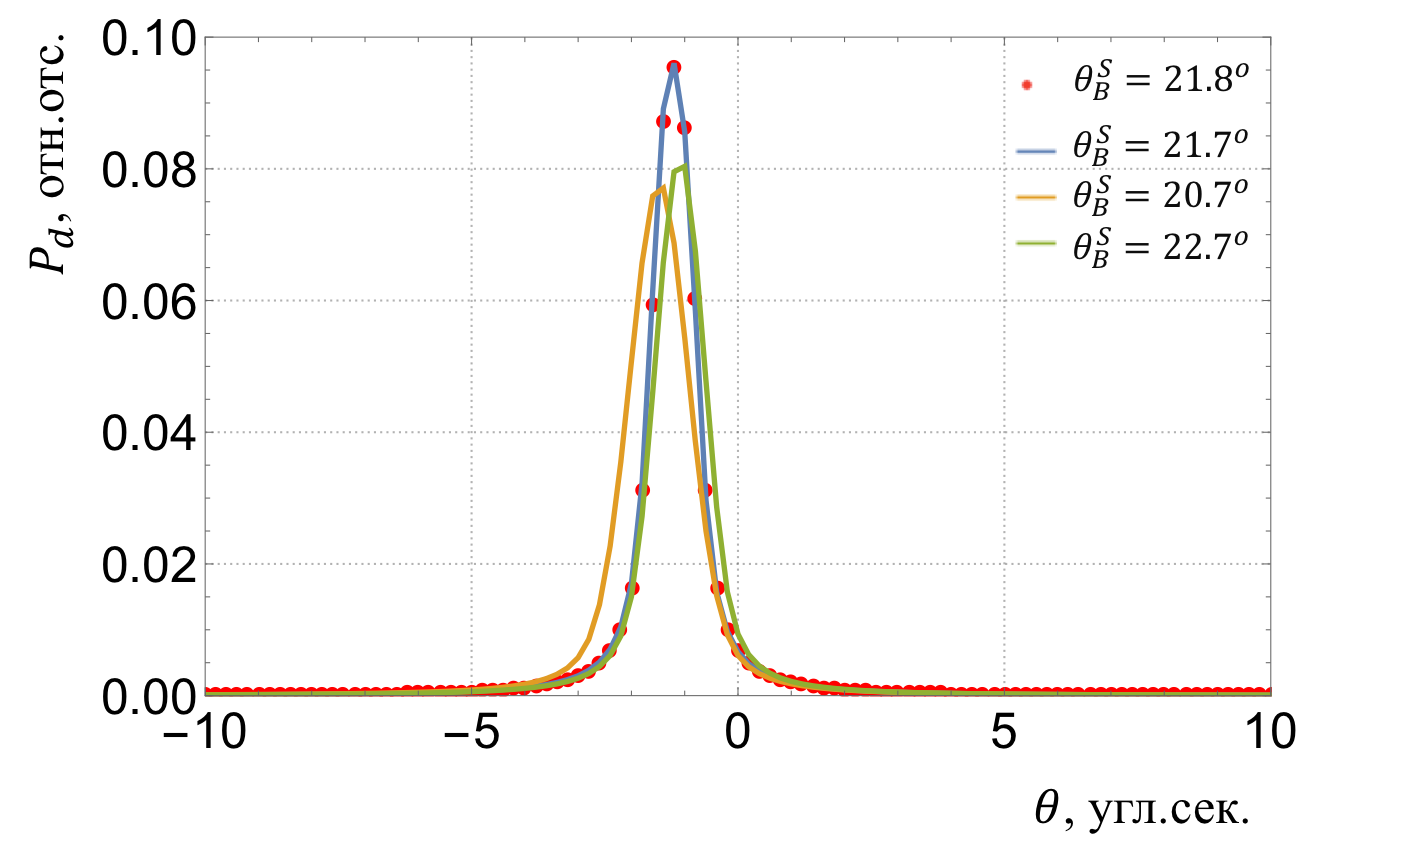
\includegraphics[width=0.8\textwidth]{images/FWHM_diference_bragg_KDO.png}
  \caption{КДО для разныой степени дисперсионности схемы, $\theta_B^M = 21.6785 ^o$}
  \label{ris:FWHM_diference_bragg_KDO}
\end{figure}

Для того, чтобы добиться существенного изменения изменения кривой нужно
иметь угловую отстройку порядка градуса, такое изменение угла Брэгга
соответсвует изменению межплоскостного расстояния на величину $d/d_0 \simeq 0.03$
процентов, а такие деформации в кристалле не допустимы (при $d/d_0 > 10^{-4}$ происходит разрушение).
Таким образом в результате пьезоэффекта профиль кривой, для рассмотренных нами случаев,
должен оставаться постоянным.

Необходимо отметить, что деформации профиля КДО может происходить вследствие наличия
заряженных дефектов в кристалле, которые подвержены влиянию электрического поля. Но данный механизм
также не рассматривается в данной работе.

Данное заключение позволяется применять рассмотренные методы расчета для определения пьезоэлектрических констант,
а так же использовать времяразрешающий метод исследования (см. \ref{sec:slope_diff_piezo}).
